% axi-scramjet.tex

\newpage
\section{Axi-symmetric Scramjet}
\label{chapter3-axi-scramjet}
%

The second example given is that of an axi-symmetric scramjet duct with a 3-ramp inlet. The purpose of this example is simply to illustrate the use and advantages of the space marching solver and as such, great detail of the model will not be given. The geometry is as shown in Figure \ref{fig:scramjet_geom} and the inflow condition is representative of Mach 8 flight at 27km altitude. 

\begin{figure}[h]
 \centering
 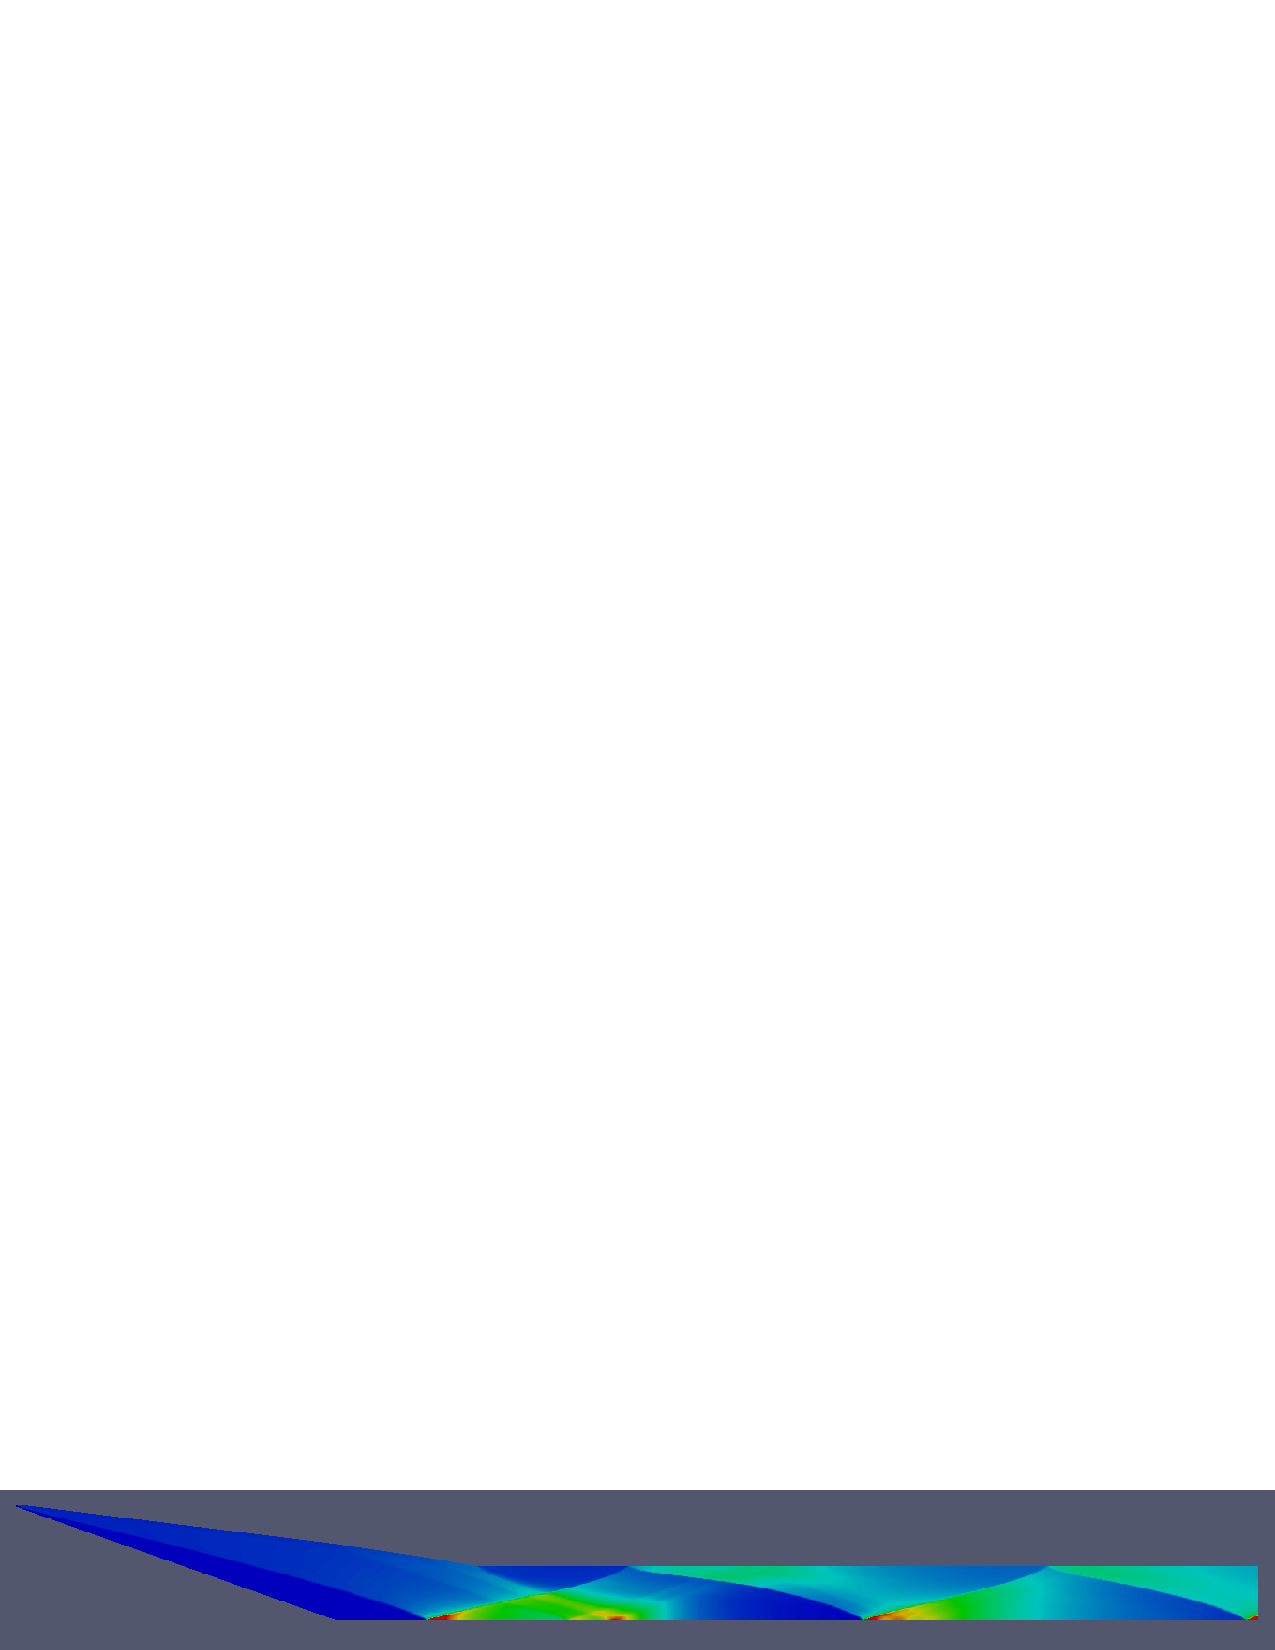
\includegraphics[width=0.9\linewidth]{./chap3-axi-scramjet/pressure_contour.pdf}
 % pressure_contour.pdf: 0x0 pixel, 300dpi, 0.00x0.00 cm, bb=
 \caption{Pressure contour of Scramjet model}
 \label{fig:scramjet_geom}
\end{figure}


The simulation was constructed with two SuperBlocks splitting the model into two different sections: 1) the inlet ramp section with 1400 axial cells and 150 sub-blocks; and 2) the combustor region with 3000 axial cells and 350 sub-blocks. The mesh used was quite fine in this example and clustered to the nose, wall and centreline.

This test case has been used to reference the current space marching solver against different simulations using the original space marching solver and the time-dependent solver. The reference for the comparison is the temperature profile down the axis of the model. Shown in figure \ref{fig:T_plot} are the centreline temperature plots for the three different cases mentioned and additionally the new space marching solver run to 6 flow lengths as a check to see whether 3 flow lengths was enough for convergence.

\begin{figure}[h]
 \centering
 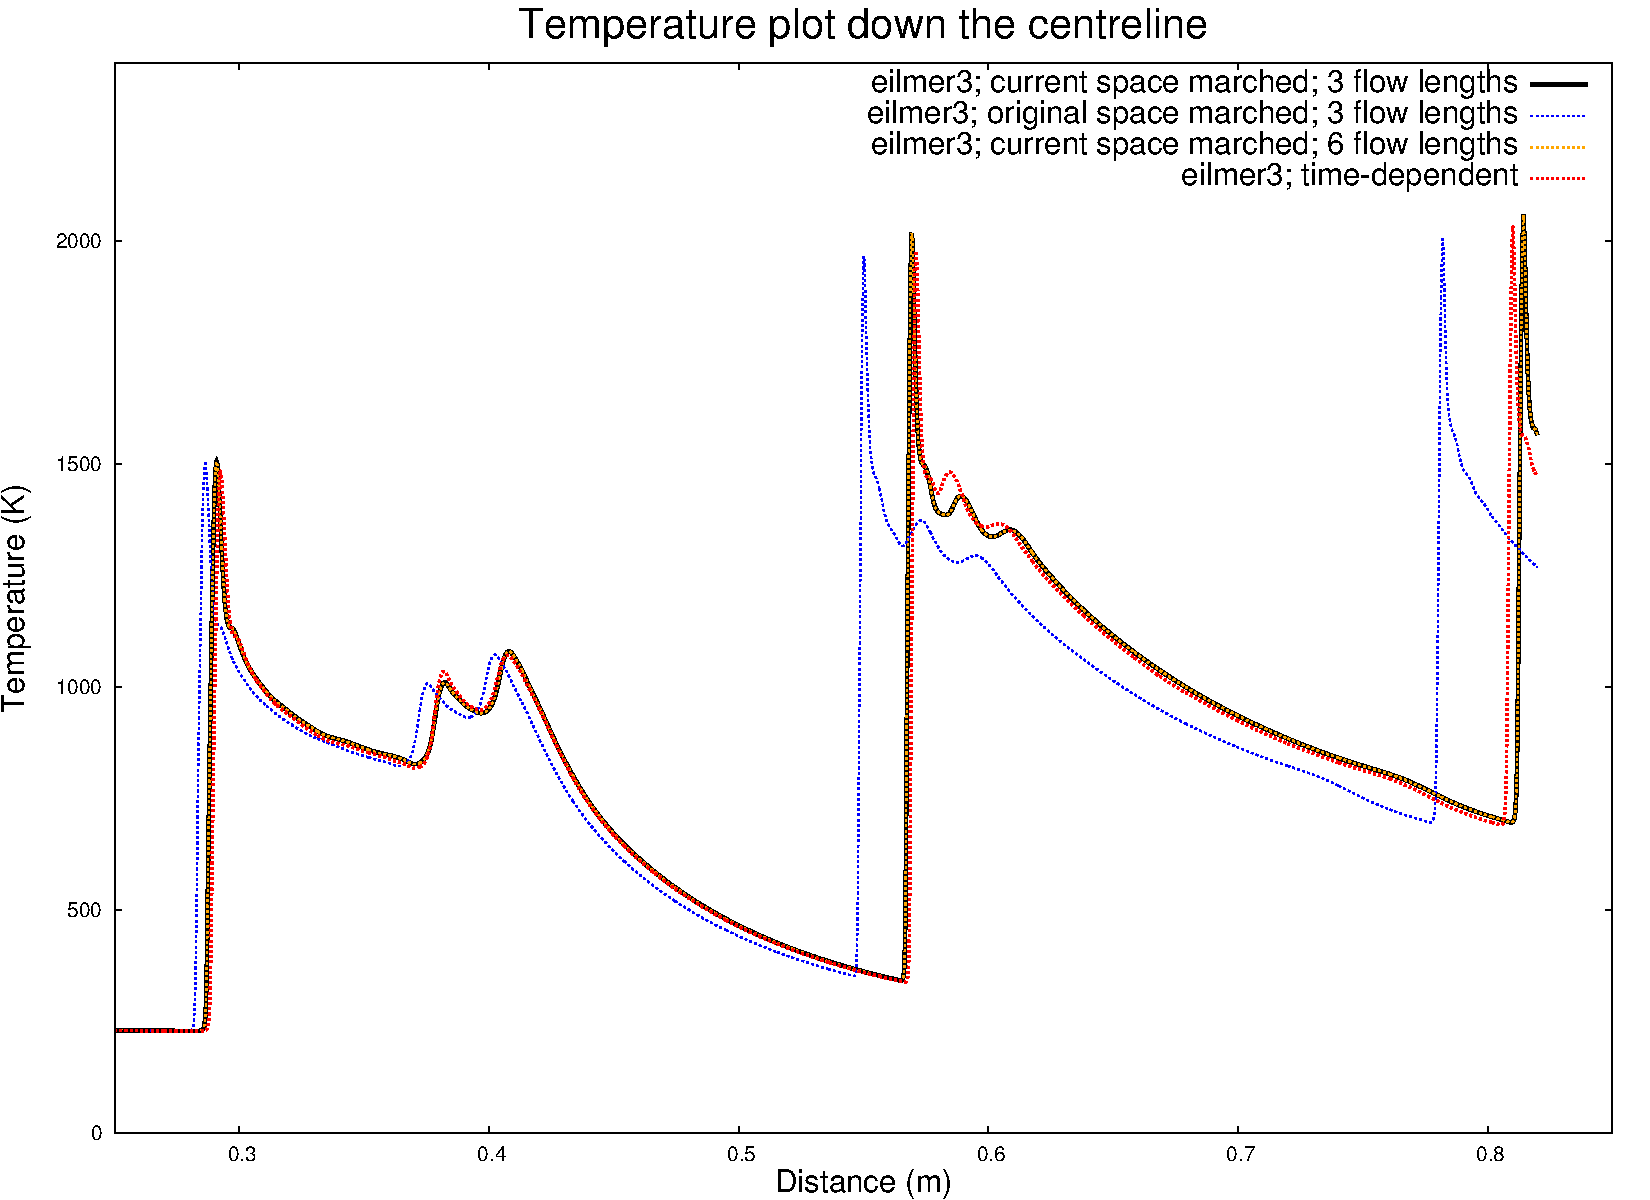
\includegraphics[width=0.9\linewidth]{./chap3-axi-scramjet/T_profile_centreline.pdf}
 % T_profile_centreline.pdf: 792x576 pixel, 72dpi, 27.94x20.32 cm, bb=0 0 792 576
 \caption{Temperature plot down the centreline}
 \label{fig:T_plot}
\end{figure}

The main points to be taken from this plot are the comparisons with the different cases. Firstly, the most noticeable difference is the comparison with the original space marching solver - the spikes have shifted noticeably downstream for the current space marching solver and now matches the results of the time-dependent solver. The previous discrepancy occurred due to the boundary data transfer between the blocks and this shows that the fix that was implemented appears to be working well. Two different computations were completed with the new space marching solver to get an indication of the effect of total simulation time however there is no appreciable difference between 3 and 6 flow lengths. 

Secondly, the other difference that can be seen in the plots occurs at approximately 0.6\,m where the space marched solver and the time resolved solver show slightly different results. This is probably due to a separation occuring in the flow which is not picked up properly by the space marching solver. The final result however is still quite close giving confidence in the use of the space marching solver for preliminary computations.